\section{Testing}
\begin{multicols}{2}

\subsection{Allgemeine Begriffe}
\begin{itemize}
	\item Definition: Programm mit der Absicht ausführen, Fehler zu finden
	\item Durch das Testen kann die Korrektheit eines Programms nicht bewiesen werden!
	\item Erster Bug: 1947 wurde eine Motte im Relais eines Mark II Aiken Rechners entdeckt.
\end{itemize}

\subsubsection{Wahrscheinlichkeit von Fehlern}
Je mehr Fehler gefunden werden, desto höher ist die Wahrscheinlichkeit weiterer Fehler.
\begin{center}
	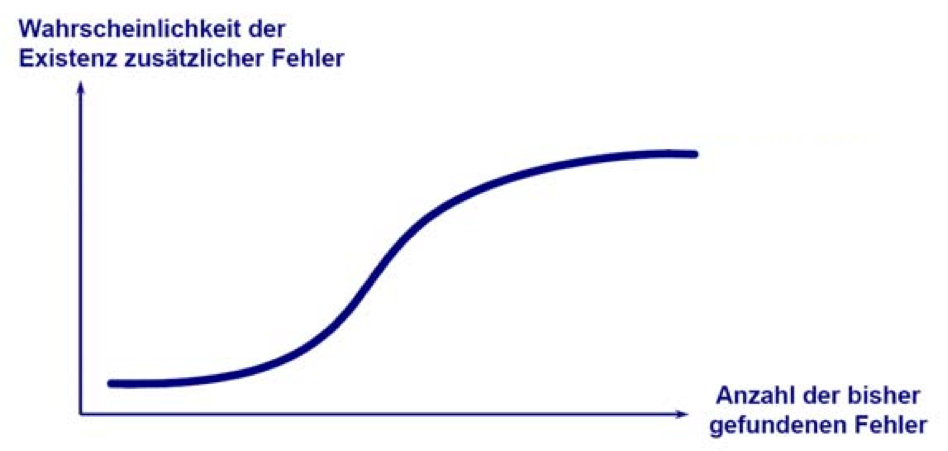
\includegraphics[width=7.5cm]{images/fehler_wkeit.png}
\end{center}

\subsubsection{Ziel}
\textbf{Ziel des Testing:} \\
Aufzeigen, dass Fehler existieren \\

\textbf{Ziel des Debugging:} \\
Durch Testing gefundene Fehler lokalisieren und beheben. \\

\subsubsection{Anforderungen}
\begin{itemize}
	\item Geplant $\rightarrow$ Testplan erstellen
	\item Systematisch $\rightarrow$ Testspezifikationen erstellen
	\item Festgehalten $\rightarrow$ Testprotokoll erstellen
	\item Reproduzierbarkeit:
			\begin{itemize}
				\item Wissen, was getestet wurde
				\item Unabhängig von testender Person
			\end{itemize}
	\item Automatisierung, wenn möglich
	\item Testspezifikationen laufend erweitern, Regressionstests
\end{itemize}

\subsubsection{Arten von Tests}
\begin{itemize}
	\item Funktionale Tests
	\item Nicht-Funktionale Tests
			\begin{itemize}
				\item Leistungstests
				\item Usability Tests
				\item ...
			\end{itemize}
\end{itemize}

\subsubsection{Massnahmen zur Softwareprüfung}
\begin{itemize}
	\item Dynamische Prüfung
			\begin{itemize}
				\item Testing
				\item Dynamische Analyse
			\end{itemize}
	\item Statische Prüfung
			\begin{itemize}
				\item Metrikanalyse
				\item Code Reviews
			\end{itemize}
\end{itemize}

\subsubsection{Wer Testet}
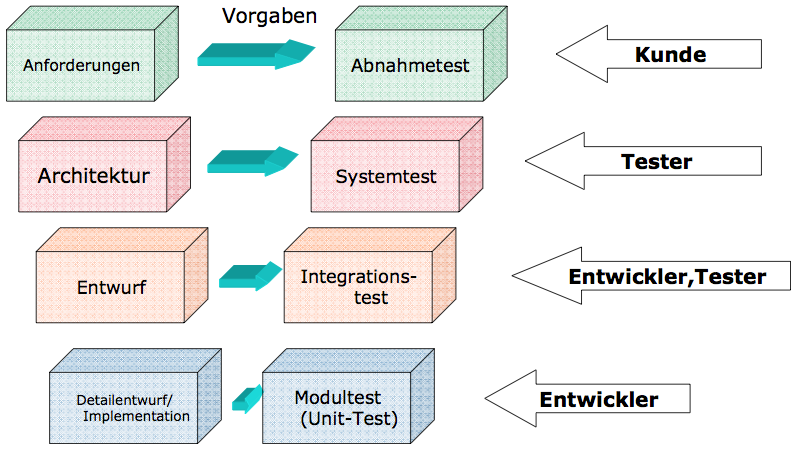
\includegraphics[width=8cm]{images/wer_testet.png}

\subsubsection{Verifikation und Validierung}
\textbf{Validierung:}\\
\textit{``Are we building the right product?''} \\

\textbf{Verifikation:} \\
\textit{``Are we building the product right?''} \\

\newpage

\subsection{Methoden}
\subsubsection{Blackbox Tests}
Tests ohne Kenntnis der inneren Struktur; Anwendung: Abnahme-, System-, Integrationstests \\

\textbf{Äquivalenzklassen:} \\
Wertebereich, für welche das Programm voraussichtlich das gleiche Verhalten zeigt. \\
Methodik: 1 Testcase pro Äquivalenzklasse \\
Beispiel: Quadratische Gleichung; Determinante $<0$ ; $=0$ ; $>0$ \\

\textbf{Grenzwertanalyse:} \\
Fehler liegen oft an Grenzen zulässiger Eingabewertbereiche. \\
Methodik: Testfälle auf Grenzen und knapp daneben \\

\textbf{Zustandsbasiertes Testing:} \\
Beispiel Stack: \\
Zustände: Stack leer, Stack halb-voll, Stack voll \\
Testfälle: Element hinzufügen, Element entfernen \\

\subsubsection{Whitebox Tests}
Tests mit Kenntnis der inneren Struktur; Anwendung: Modul-, Integrationstests \\

\textbf{Kontrollfluss-orientiertes Testen:} \\
Erstellen eines Kontrollfluss-Graphen, in welchem jedes Statement einem Knoten entspricht. Zweige, welche Schleifen und Verzweigungen entsprechen, verbinden die Knoten. Der Test wird so ausgelegt, dass die Überdeckung (Coverage) möglichst gut ist. (Test der Überdeckung mit Dynamic Analyzer) \\

\begin{itemize}
	\item Anweisungsüberdeckung
			\begin{itemize}
				\item Prozentualer Anteil der Anweisungen im Test ausführen
				\item 100\% Anweisungsüberdeckung ist Minimum
			\end{itemize}
	\item Zweigüberdeckung
			\begin{itemize}
				\item Prozentualer Anteil der Zweige wird durchlaufen
				\item 100\% Zweigüberdeckung $\Rightarrow$ 100\% Anweisungsüberdeckung
				\item Da 100\% kaum erreichbar werden oft Äquivalenzklassen u/o Grenzwerte auf Kontrollstrukturen angewandt
			\end{itemize}
	\item Bedingungsüberdeckung
			\begin{itemize}
				\item Verschiedene Kombinationen testen bei Verzweigungen
				\item mind. 1x true/false durchlaufen
			\end{itemize}
	\item Funktionsüberdeckung
			\begin{itemize}
				\item ``Tut es das, was der Kunde spezifiziert hat?''
				\item 1 Szenario pro Use Case 
				\item Blackbox Tests
			\end{itemize}
\end{itemize}

\subsection{Automatisiertes Testing}
Vorteile:
	\begin{itemize}
		\item Wiederholbarkeit (Regressionstests möglich)
		\item Eindeutige Spezifikationen (Testcode ist Programmcode)
	\end{itemize}
	
Nachteile:
	\begin{itemize}
		\item Mehr Code zu schreiben und pflegen
		\item Testcode ist Programmcode: Wird überhaupt das Richtige getestet?
	\end{itemize}
	
\subsection{Testwerkzeuge}
\begin{tabular}{ll}
	Blackbox: & FIT \\
	Whitebox: & xUnit
\end{tabular}

\end{multicols}